% Options for packages loaded elsewhere
\PassOptionsToPackage{unicode}{hyperref}
\PassOptionsToPackage{hyphens}{url}
\PassOptionsToPackage{dvipsnames,svgnames,x11names}{xcolor}
%
\documentclass[11pt]{article}
\usepackage{amsmath,amssymb}
\usepackage{lmodern}
\usepackage{iftex}
\ifPDFTeX
  \usepackage[T1]{fontenc}
  \usepackage[utf8]{inputenc}
  \usepackage{textcomp}
\fi
\IfFileExists{microtype.sty}{\usepackage[]{microtype}\UseMicrotypeSet[protrusion]{basicmath}}{}
\makeatletter
\@ifundefined{KOMAClassName}{%
  \IfFileExists{parskip.sty}{\usepackage{parskip}}{%
    \setlength{\parindent}{0pt}\setlength{\parskip}{6pt plus 2pt minus 1pt}}
}{\KOMAoptions{parskip=half}}
\makeatother
\usepackage{xcolor}
\IfFileExists{xurl.sty}{\usepackage{xurl}}{}
\IfFileExists{bookmark.sty}{\usepackage{bookmark}}{\usepackage{hyperref}}
\hypersetup{
  pdftitle={Final Report, Indoor Air Quality (CO2) Management},
  pdfauthor={Oscar Lundqvist Engelmark},
  colorlinks=true,
  linkcolor={RoyalBlue},
  filecolor={Maroon},
  citecolor={Blue},
  urlcolor={Blue}}
\urlstyle{same}
\usepackage[a4paper,margin=2.4cm]{geometry}
\usepackage{longtable,booktabs,array}
\usepackage{calc}
\usepackage{graphicx}
\makeatletter
\def\maxwidth{\ifdim\Gin@nat@width>\linewidth\linewidth\else\Gin@nat@width\fi}
\def\maxheight{\ifdim\Gin@nat@height>\textheight\textheight\else\Gin@nat@height\fi}
\makeatother
\setkeys{Gin}{width=\maxwidth,height=\maxheight,keepaspectratio}
\setlength{\emergencystretch}{3em}
\providecommand{\tightlist}{\setlength{\itemsep}{0pt}\setlength{\parskip}{0pt}}
\setcounter{secnumdepth}{-\maxdimen}
\usepackage{newunicodechar}
\usepackage{textcomp}
\usepackage{amssymb}
\newunicodechar{°}{\textdegree}
\newunicodechar{₂}{\textsubscript{2}}
\newunicodechar{→}{\ensuremath{\rightarrow}}
\newunicodechar{≤}{\ensuremath{\leq}}
\newunicodechar{≥}{\ensuremath{\geq}}
\newunicodechar{≈}{\ensuremath{\approx}}
\newunicodechar{✓}{\ensuremath{\checkmark}}
\newunicodechar{–}{--}
\newunicodechar{—}{---}
\usepackage{etoolbox}
\AtBeginEnvironment{longtable}{\footnotesize}
\AtBeginEnvironment{tabular}{\footnotesize}
\usepackage{fancyhdr}
\pagestyle{fancy}\fancyhf{}
\rhead{\small D7065E\,--\,Architecture Document}
\lhead{\small Indoor Air Quality (CO\textsubscript{2}) Management}
\cfoot{\thepage}
\renewcommand{\headrulewidth}{0.4pt}
\usepackage{titlesec}
\titleformat{\section}{\Large\bfseries}{\thesection}{0.6em}{}
\titleformat{\subsection}{\large\bfseries}{\thesubsection}{0.5em}{}
\usepackage{microtype}
\usepackage{pgfplots}
\pgfplotsset{compat=1.16}
\setlength{\emergencystretch}{2em}

% --- template helpers -------------------------------------------------------
\definecolor{guidegray}{gray}{0.42}
% Grey guidance note: what this section must contain. Delete before submission.
\newcommand{\guidance}[1]{{\color{guidegray}\small\textit{#1}}\par\vspace{0.3em}}
% A slot to be replaced with the team's own prose.
\newcommand{\fillin}[1]{\par\noindent\fbox{\parbox{\dimexpr\linewidth-2\fboxsep-2\fboxrule}{\color{guidegray}\textit{[#1]}}}\par\vspace{0.4em}}
% A placeholder where a rendered diagram should be inserted.
\newcommand{\diagramslot}[1]{\par\begin{center}\fbox{\parbox[c][2.6cm][c]{0.82\linewidth}{\centering\color{guidegray}\textit{[Insert: #1]}}}\end{center}\par}
% ---------------------------------------------------------------------------

\title{Indoor Air Quality (CO\textsubscript{2}) Management}
\usepackage{etoolbox}
\makeatletter
\providecommand{\subtitle}[1]{\apptocmd{\@title}{\par {\large #1 \par}}{}{}}
\makeatother
\subtitle{D7065E, Embedded Intelligence at the Edge}
\author{Oscar Lundqvist Engelmark}
\date{}

\begin{document}

\begin{center}
{\LARGE Indoor Air Quality (CO\textsubscript{2}) Management\par}
\vspace{0.5em}
{\large D7065E, Architecture Document\par}
\vspace{1em}
{Oscar Lundqvist Engelmark\par}
\end{center}

\vspace{1.2em}

{
\hypersetup{linkcolor=black}
\setcounter{tocdepth}{3}
\tableofcontents
}

\section{1. Summary}

\guidance{One short paragraph: what the system does and the single guiding
principle that threads through the design. Then the summary table, and a brief note
of what changed since the Week 2 proposal and why.}

\fillin{Write the one-paragraph summary here.}

\begin{longtable}[]{@{}
  >{\raggedright\arraybackslash}p{(\columnwidth - 2\tabcolsep) * \real{0.35}}
  >{\raggedright\arraybackslash}p{(\columnwidth - 2\tabcolsep) * \real{0.65}}@{}}
\toprule
\textbf{Field} & \textbf{Value} \\
\midrule
\endhead
\textbf{Project title} & \\
\textbf{Team members} & \\
\textbf{Use case} & \\
\textbf{Repository} & \\
\textbf{Version / date} & \\
\bottomrule
\end{longtable}

\textbf{Changes since the proposal.}
\fillin{List the design changes made since the proposal, and the evidence that
forced each one. If nothing changed, state that and say why.}

\section{2. Use case and building context}

% Required points (report guide, section 3.2; template, section 2):
% - the use case, and how it connects to BuildSim; BuildSim is not modified
% - the building and what BuildSim provides (rooms, sensors, actuators, 3D view)
% - how each process uses BuildSim
% - the actors
% - the concrete scenario the demo shows
% - why the use case matters; what makes the decision non-trivial

\textbf{The use case.} The system manages the indoor air quality of one
office room. It keeps the room's CO₂ concentration under 1000 ppm
(Section 7.1) while running the ventilation as low as it can. CO₂ rises
as the people in the room breathe and falls as ventilation replaces room
air with outdoor air. The system therefore senses one variable, CO₂, and
acts through one device: a ventilation damper whose level runs from 0
(closed) to 1 (fully open).

\textbf{The building and BuildSim.} The room is A125, on level 0 of the
LTU A-building as modelled in BuildSim, with a floor area of 29.8 m² and
room for six people. BuildSim holds the shared state of the building in memory:
its rooms and their floor areas, the devices registered in each room with
their current values, and who is in which room. Processes read and write
that state through its REST API, and a 3D view shows the building in a
browser. BuildSim is the course's own program, built from the course
repository at a fixed version and never modified. The project only adds
its own devices to it through the API: a CO₂ sensor, an occupancy sensor,
and a damper in A125.

\textbf{How the processes use BuildSim.} Five of the project's processes
talk to BuildSim. The decision service, the storage service, the room
model, and the dashboard never do.

\begin{itemize}
\tightlist
\item
  \textbf{The occupancy simulator and the physical model} stand in for the
  physical world (Section 6). The occupancy simulator writes who is in each
  room (\texttt{PUT /api/occupancy}). The physical model reads the people
  in the room, the damper's state, and the current CO₂, steps the CO₂
  forward, and writes the result as the CO₂ sensor's value
  (\texttt{PUT /api/sensors/\{id\}/value}). It is the only process that
  changes the CO₂, and its reading of the damper is what closes the loop.
\item
  \textbf{The CO₂ sensor} reads its sensor's value
  (\texttt{GET /api/sensors/\{id\}}) and publishes it to the MQTT message
  broker. Like a real sensor, it reports the room's CO₂ but does not
  produce it.
\item
  \textbf{The occupancy sensor} reads who is in the room
  (\texttt{GET /api/occupancy}), writes the head count as its own device's
  value, and publishes it to the broker.
\item
  \textbf{The damper actuator} receives the decision service's commands
  over REST and writes each new level to the damper
  (\texttt{PUT /api/actuators/\{id\}/state}). BuildSim is the one place
  the damper's position is kept.
\end{itemize}

BuildSim starts with no devices, so the CO₂ sensor, the occupancy sensor,
and the damper actuator each register their own device when they start
(\texttt{POST /api/equipment/bulk}).

\textbf{Actors.} The \textbf{operator} watches the room's CO₂, head count,
and damper level on the dashboard (Section 12), which reads the stored
history rather than BuildSim. The \textbf{room's occupants} raise the CO₂
by being in the room; here they are simulated from a weekday schedule
(Section 6). Neither is on the control path: the loop runs without anyone
acting on it.

\textbf{The scenario the demo shows.} For most of a weekday, three people
work in A125. At 13:00 a meeting fills the room to its six-person maximum
for an hour. This is the case where CO₂ climbs fast enough to cross
1000 ppm, so it is the one the decision service has to hold under the
threshold. The occupancy sensor reports six, and the decision service
raises the damper to the lowest level its room model predicts will hold
six people under the threshold. When the meeting ends, the level drops
back. Room time can run faster than the wall clock, so the demo shows the
whole meeting in a few minutes. Section 11 reports whether the threshold
holds.

\textbf{Why it matters.} The system's goals pull against each other. The
ventilation must be able to hold a full room under 1000 ppm, since a room
can fill without warning, yet for most of the day A125 holds three people
or none. Running the ventilation at the full-room setting all day keeps
the air fresh at a cost in noise and energy. A fixed low setting is quiet
but lets CO₂ pass the threshold when the meeting fills the room. The level
that meets both depends on how many people are in the room now and on how
this particular room responds to people and to ventilation. That is what
makes the decision worth automating: the system counts the people and
learns the room's response from its own stored data (Section 7.1).

\section{3. Requirements}

\guidance{List functional and non-functional requirements with stable IDs, so each
can be traced to a test in the test plan and to results in the evaluation. Keep them
verifiable (avoid ``fast'' or ``reliable'' without a number).}

\begin{longtable}[]{@{}
  >{\raggedright\arraybackslash}p{(\columnwidth - 4\tabcolsep) * \real{0.12}}
  >{\raggedright\arraybackslash}p{(\columnwidth - 4\tabcolsep) * \real{0.58}}
  >{\raggedright\arraybackslash}p{(\columnwidth - 4\tabcolsep) * \real{0.30}}@{}}
\toprule
\textbf{ID} & \textbf{Requirement} & \textbf{How it is verified} \\
\midrule
\endhead
FR-1 & & \\
FR-2 & & \\
NFR-1 & & \\
NFR-2 & & \\
\bottomrule
\end{longtable}

\section{4. Architecture}

\subsection{4.1 Context diagram (C4 Level 1)}

\guidance{The system as a single box, with the people and external systems it
interacts with (including BuildSim). One paragraph of narrative explaining the
boundaries and the main interactions.}

\diagramslot{Context diagram (C4 Level 1)}

\fillin{Narrative for the context diagram.}

\subsection{4.2 Container diagram (C4 Level 2)}

\guidance{Open the system into its separately-running parts (sensor services,
autonomous service, actuators, storage, dashboard) and how they communicate. Explain
why the system is split this way.}

\diagramslot{Container diagram (C4 Level 2)}

\fillin{Narrative for the container diagram.}

\subsection{4.3 Component diagram (C4 Level 3)}

\guidance{Zoom into one container that is worth explaining (often the autonomous
service) and show its internal components and their responsibilities.}

\diagramslot{Component diagram (C4 Level 3)}

\fillin{Narrative for the component diagram.}

\subsection{4.4 Design decisions and alternatives}

\guidance{The core of the architecture grade. For each significant decision, state
the choice, the alternatives considered, and the evidence or reasoning for choosing
it over them. A decision with no rejected alternative is not yet justified.}

\begin{longtable}[]{@{}
  >{\raggedright\arraybackslash}p{(\columnwidth - 4\tabcolsep) * \real{0.25}}
  >{\raggedright\arraybackslash}p{(\columnwidth - 4\tabcolsep) * \real{0.35}}
  >{\raggedright\arraybackslash}p{(\columnwidth - 4\tabcolsep) * \real{0.40}}@{}}
\toprule
\textbf{Decision} & \textbf{Alternatives considered} & \textbf{Why this one} \\
\midrule
\endhead
 & & \\
 & & \\
 & & \\
\bottomrule
\end{longtable}

\section{5. Interfaces and data contracts}

\guidance{The contracts between components: API endpoints and/or message topics,
with payload schemas and an example message. Precise enough that a component could be
re-implemented from this section alone.}

\fillin{Define the interfaces and data contracts here (endpoints/topics, schemas,
example payloads).}

\section{6. Simulating the sensor values (the physical model)}

\guidance{How sensor values are produced. State the per-room physical model
(temperature heat balance, CO₂ from occupancy and ventilation) and, critically, how
actuator commands feed back so the control loop closes. Include the occupancy model
(for example, a head-count per room sampled conditional on room type and time of day).
Give the governing equations.}

\fillin{Describe the physical and occupancy models, with equations, here.}

\section{7. Autonomous services and data pipeline}

\subsection{7.1 The autonomous service}

\guidance{The decision logic: inputs, the algorithm or rules, and outputs. Rule-based
control is fully acceptable if justified; if a learned model is used, explain training,
data, and the fallback when data is thin.}

\fillin{Describe the autonomous service here.}

\subsection{7.2 The data pipeline}

\guidance{How readings are collected, stored, and served to the autonomous service
and the dashboard. State what is retained and for how long.}

\fillin{Describe the data pipeline here.}

\section{8. Behaviour}

\subsection{8.1 Key scenario (dynamic diagram)}

\guidance{Walk one important scenario end-to-end (for example, a room filling up) as
a C4 dynamic / sequence diagram, with a short narrative of the message order.}

\diagramslot{Dynamic / sequence diagram for the key scenario}

\fillin{Narrative for the key scenario.}

\subsection{8.2 Process lifecycle (state diagram)}

\guidance{The lifecycle of a key process or zone (for example, setback $\rightarrow$
active $\rightarrow$ fault), as a state diagram with the transitions.}

\diagramslot{State diagram for the process lifecycle}

\fillin{Narrative for the state diagram.}

\section{9. Deployment and component view}

\guidance{Where each process runs (edge nodes, a server, BuildSim) and how they are
connected. Note where computation belongs and why.}

\diagramslot{Deployment diagram}

\fillin{Narrative for the deployment view.}

\section{10. Test plan}

\guidance{The tests that verify the requirements, including stress and failure tests
(a sensor that lies, a process that dies, a flood of readings). Each row should trace
back to a requirement ID from Section 3.}

\begin{longtable}[]{@{}
  >{\raggedright\arraybackslash}p{(\columnwidth - 6\tabcolsep) * \real{0.16}}
  >{\raggedright\arraybackslash}p{(\columnwidth - 6\tabcolsep) * \real{0.40}}
  >{\raggedright\arraybackslash}p{(\columnwidth - 6\tabcolsep) * \real{0.19}}
  >{\raggedright\arraybackslash}p{(\columnwidth - 6\tabcolsep) * \real{0.25}}@{}}
\toprule
\textbf{ID} & \textbf{Test} & \textbf{Requirement} & \textbf{Expected result} \\
\midrule
\endhead
T-1 & & & \\
T-2 & & & \\
T-3 (stress) & & & \\
\bottomrule
\end{longtable}

\section{11. Evaluation and results}

\guidance{The evidence that the system works, measured, not asserted. Charts and
tables of results, compared against the requirements. Include an honest reading of
where the numbers are weak. The plot below is a pgfplots placeholder, replace the
coordinates with real data.}

\begin{center}
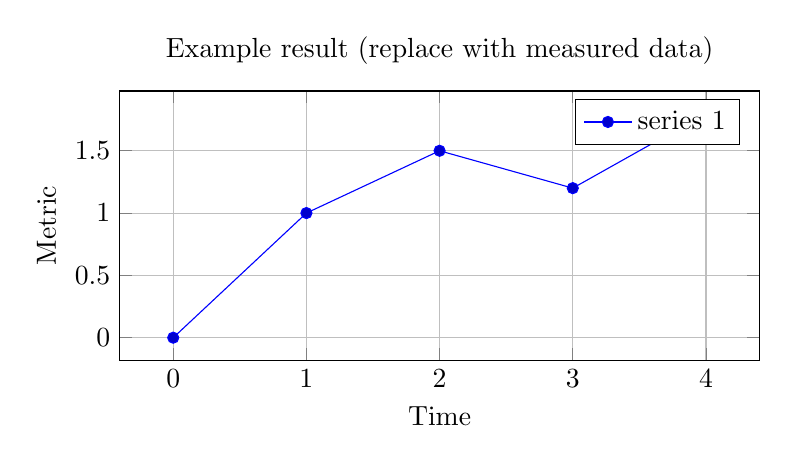
\begin{tikzpicture}
\begin{axis}[width=0.8\linewidth,height=5cm,xlabel={Time},ylabel={Metric},
  title={Example result (replace with measured data)},grid=both,
  legend pos=north east]
\addplot coordinates {(0,0) (1,1) (2,1.5) (3,1.2) (4,1.8)};
\legend{series 1}
\end{axis}
\end{tikzpicture}
\end{center}

\fillin{Present and interpret the results here.}

\section{12. Dashboard}

\guidance{What the dashboard shows and how it overlays state and decisions on the
BuildSim 3D view. Include a screenshot.}

\diagramslot{Dashboard screenshot}

\fillin{Describe the dashboard here.}

\section{13. Risks and critical reflection}

\guidance{An honest account of weaknesses, trade-offs, and what would be done with
more time. Critical thinking is graded here: naming a real limitation scores better
than claiming there are none.}

\fillin{Reflect critically on the design here: limitations, trade-offs, and next
steps.}

\section{Checklist before submission}

\begin{itemize}
\tightlist
\item All \textcolor{guidegray}{\textit{[bracketed slots]}} replaced with real content.
\item All grey guidance notes deleted.
\item All five diagrams inserted and referenced in the text (context, container, component, dynamic, deployment).
\item Every requirement in Section 3 traced to a test in Section 10.
\item Each design decision in Section 4.4 names a rejected alternative.
\item Evaluation backed by measured data, not assertions.
\item The document matches what was actually built.
\end{itemize}

\end{document}
